\chapter{実験}
\label{implementation}

\section{実験環境}
本実験では、理想的なボディビルのポーズを実現するために、特定の関節角度を有する3Dモデルを用いた。具体的には、ダブルバイセップスとクラシックポーズの2つのポーズを選定し、それぞれに対して3Dモデルを作成した。ダブルバイセップスのポーズでは、モデルの両肘は75度、両肩は160度に設定され、図\ref{fig:pose1}に示されている。一方、クラシックポーズでは、右肘が75度、左肘が180度、右肩が175度、左肩が165度に設定され、図\ref{fig:pose2}にて視覚化されている。

\begin{figure}[H]
\begin{center}
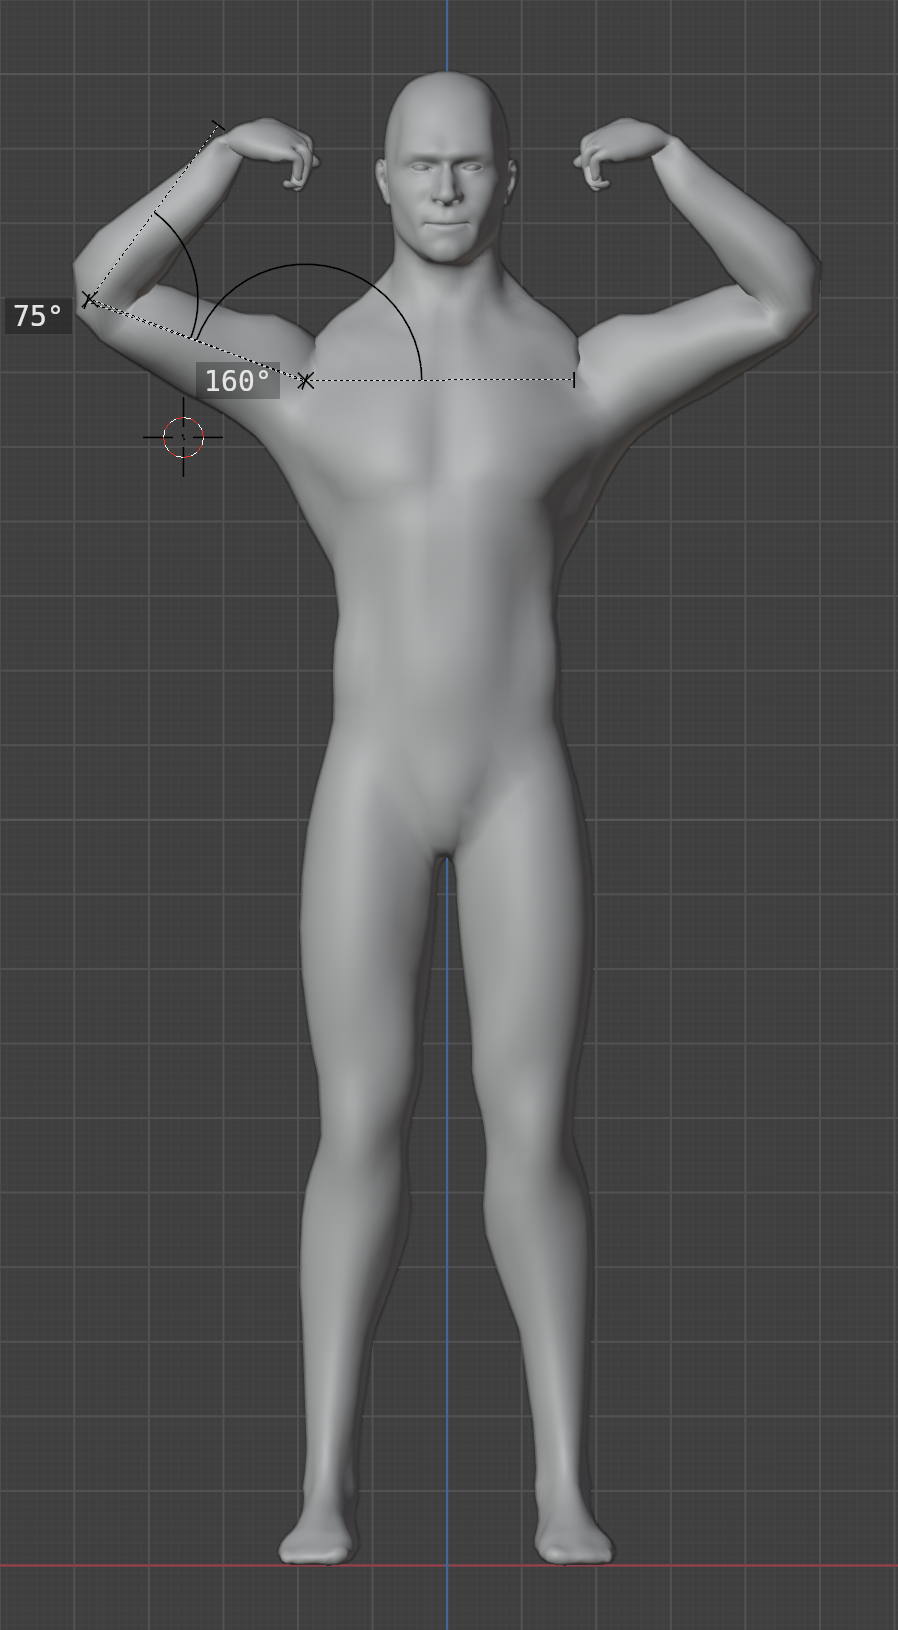
\includegraphics[width=6.5cm]{figures/pose1.png}
\caption{ダブルバイセップス(pose1)}
\label{fig:pose1}
\end{center}
\end{figure}
\begin{figure}[H]
\begin{center}
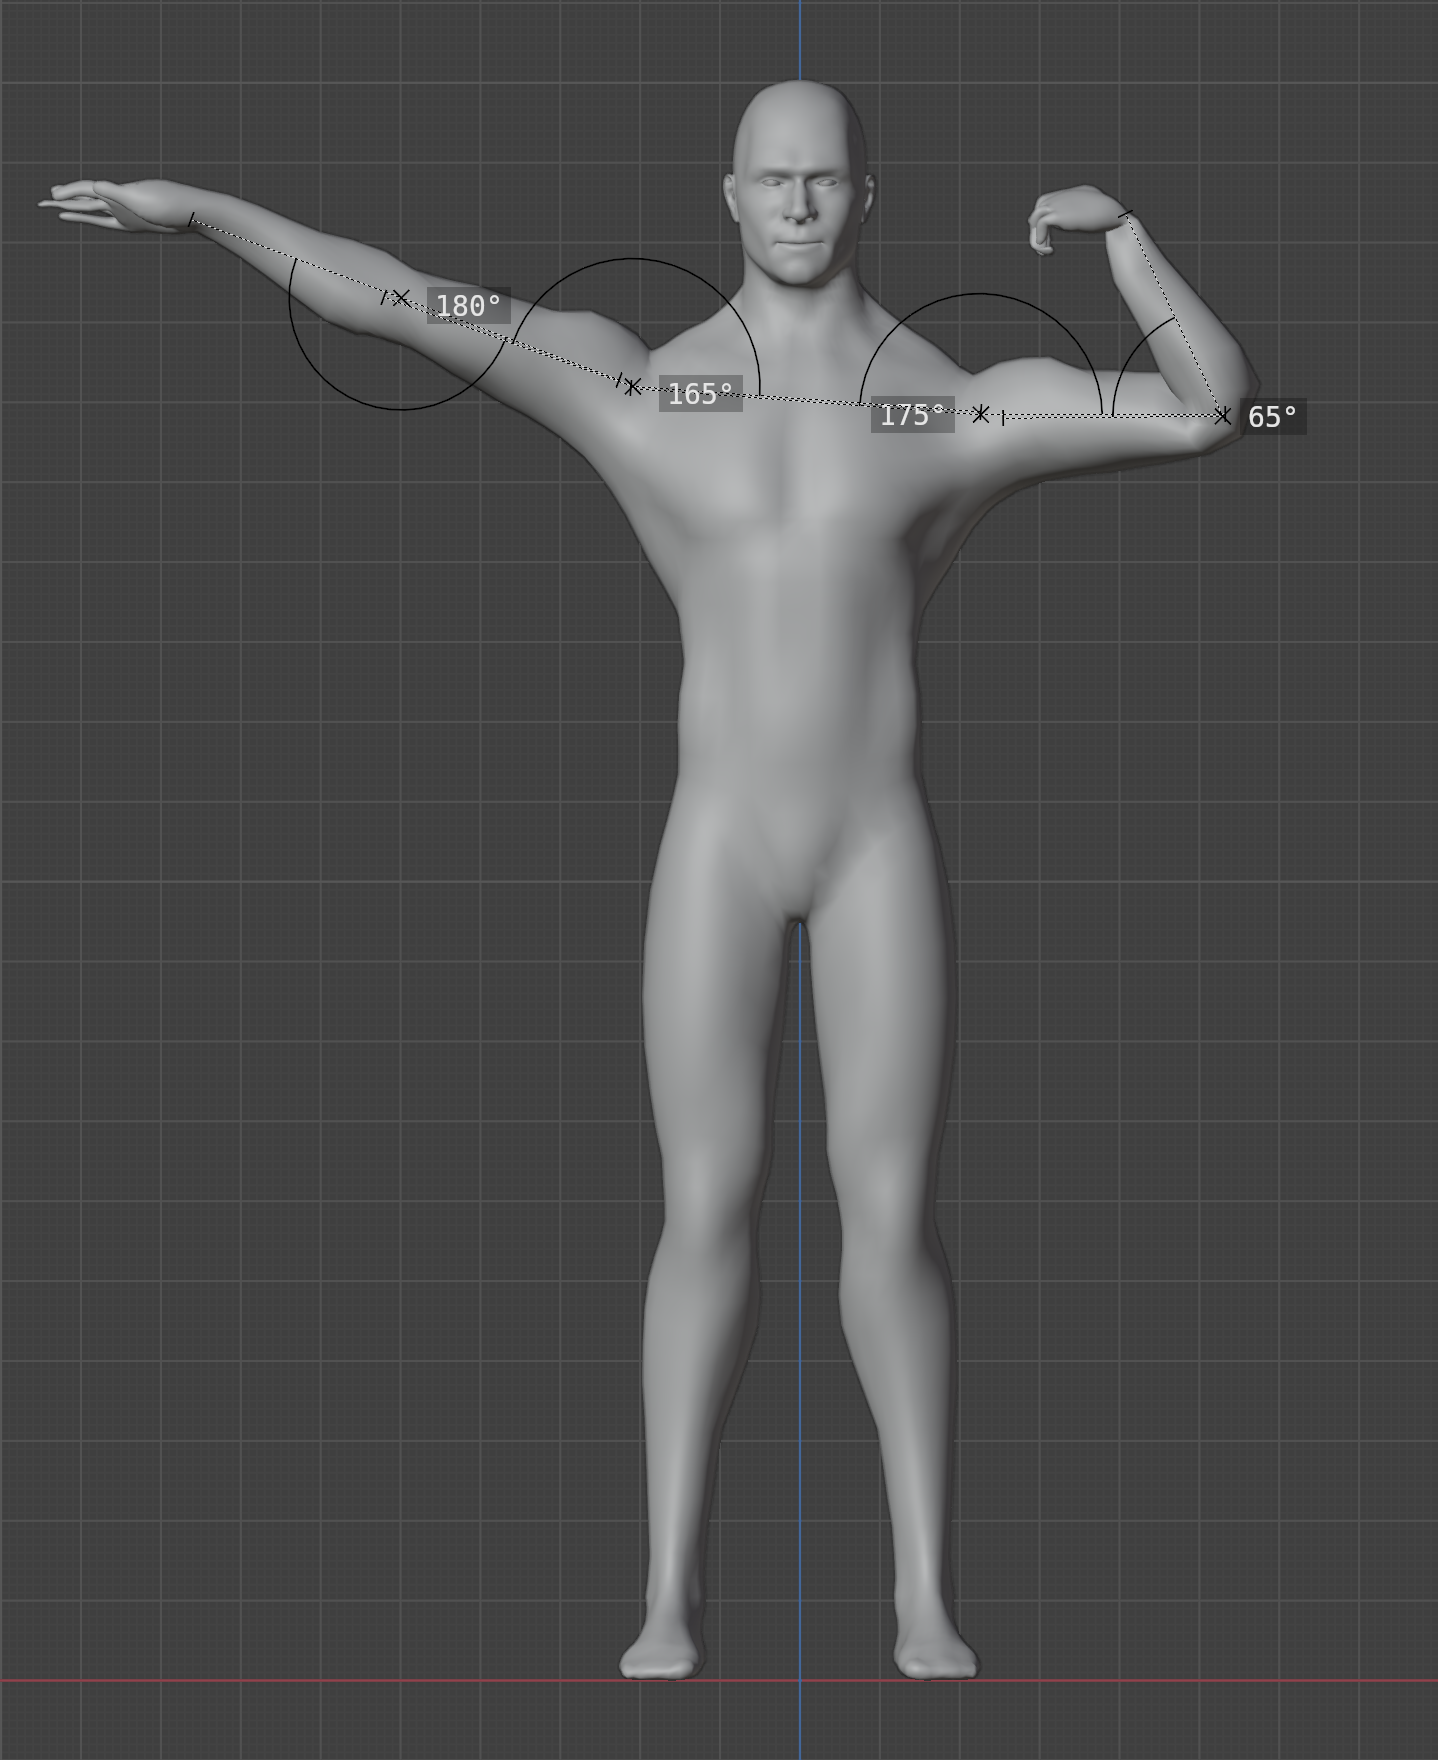
\includegraphics[width=6.5cm]{figures/pose2.png}
\caption{クラシックポーズ(pose2)}
\label{fig:pose2}
\end{center}
\end{figure}

被験者は2つのグループに分けられた。グループ1の被験者は、pose1を本実験で使用するシステムを利用して練習し、pose2は鏡を使用して練習した。対照的に、グループ2の被験者はpose1を鏡を用いて練習し、pose2は本システムを用いて練習することとした。

両グループの被験者には、システムを使用する練習と鏡を使用する練習をそれぞれ行ってもらい、各ポーズを30秒間保持すること、その後30秒間休憩することを1セットとし、合計10セットを完了させた。
システム、鏡どちらを使用して練習する場合でも理想のポーズとして図\ref{fig:pose1},図\ref{fig:pose2}を視認できる状態にた。
システム利用時にはシステムの音声に従ってポーズを修正するように指示し、鏡利用時には鏡の像と理想のポーズとしてみている図とを比較しポーズを修正するように指示をした。

被験者のポーズは練習前、練習後、練習から24時間後に計測した。図\ref{fig:schedule}

\begin{figure}[H]
\begin{center}
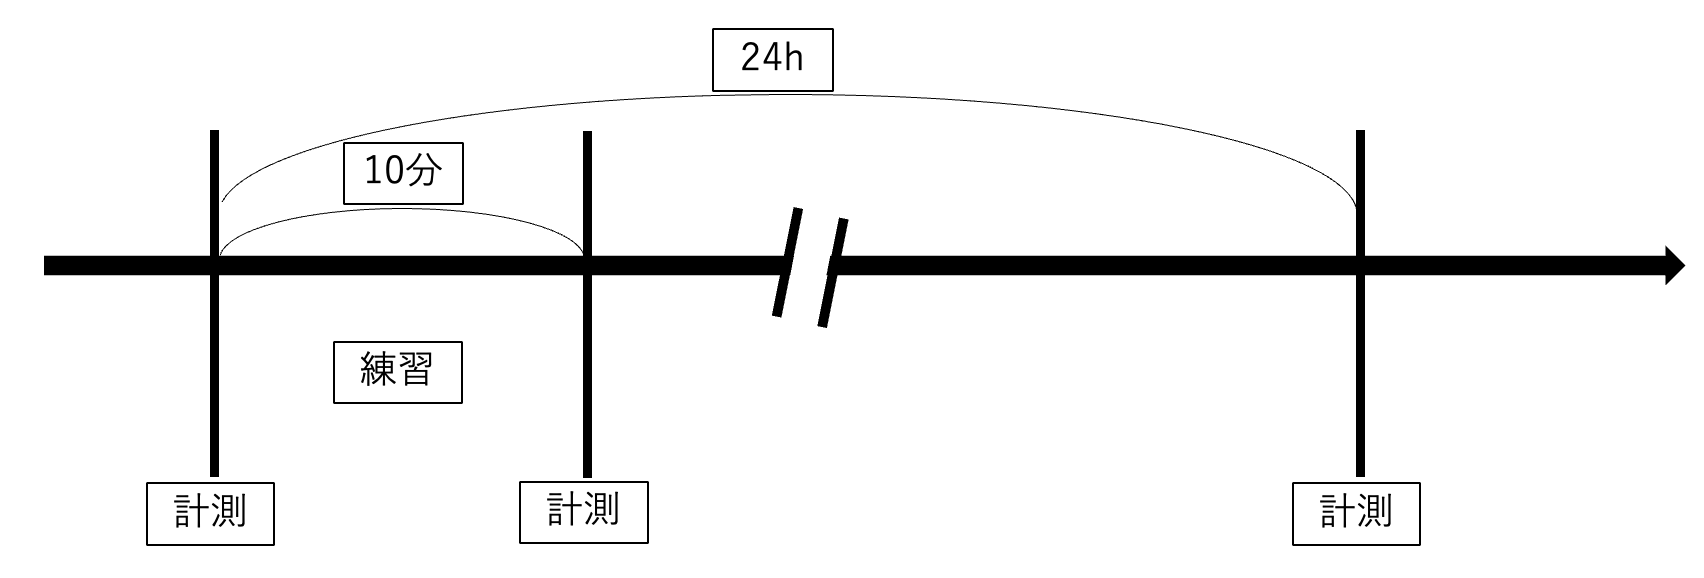
\includegraphics[width=9cm]{figures/schedule.png}
\caption{実験のスケジュール}
\label{fig:schedule}
\end{center}
\end{figure}